%% ============================================================
%% Article — Sustainable Energy Technologies and Assessments (SETA)
%% AHSE: Adaptive Honest Selection Ensemble with Clearness-Index
%%       Gating for Multi-Horizon Photovoltaic Power Forecasting
%%
%% Author   : Bilali Boureima Cissé
%% Target   : SETA (Elsevier, Q1, IF ~8.67, ISSN 2213-1388)
%% Template : Elsevier CAS Standard (elsarticle)
%% ============================================================

\documentclass[preprint,12pt]{elsarticle}

%% ------------------------------------------------------------
%% Core packages
%% ------------------------------------------------------------
\usepackage[utf8]{inputenc}
\usepackage[T1]{fontenc}
\usepackage{amsmath,amssymb}
\usepackage{graphicx}
\usepackage{booktabs}
\usepackage{array}
\usepackage{tabularx}
\usepackage{multirow}
\usepackage{siunitx}
\usepackage{xcolor}
\usepackage[hidelinks]{hyperref}
\usepackage{xurl}            % allow line breaks anywhere in long URLs
\usepackage{cleveref}

%% Algorithms — required by Section 3 (HSP pseudocode)
\usepackage[ruled,linesnumbered]{algorithm2e}
\SetKwInput{KwIn}{Input}
\SetKwInput{KwOut}{Output}

%% ------------------------------------------------------------
%% Figure path (figures live in ./figures/)
%% ------------------------------------------------------------
\graphicspath{{figures/}}

%% ------------------------------------------------------------
%% Float tuning — prevent figures from piling up at end
%% ------------------------------------------------------------
\usepackage{placeins}          % \FloatBarrier command
\renewcommand{\topfraction}{0.85}
\renewcommand{\bottomfraction}{0.50}
\renewcommand{\textfraction}{0.10}
\renewcommand{\floatpagefraction}{0.70}
\setcounter{totalnumber}{6}
\setcounter{topnumber}{4}
\setcounter{bottomnumber}{2}

%% ------------------------------------------------------------
%% Target journal (appears in preprint header)
%% ------------------------------------------------------------
\journal{Sustainable Energy Technologies and Assessments}

%% ============================================================
\begin{document}

\begin{frontmatter}

\title{Honest ensemble selection with archived weather forecasts and
       conformal intervals for photovoltaic power forecasting:
       a curtailment-aware evaluation on two sites}

\author[1,2]{Bilali Boureima Cissé}
\ead{billciss@whu.edu.cn}

\author[1,2]{Ghamgeen Izat Rashed\corref{corr}}
\ead{ghamgeen@whu.edu.cn}
\cortext[corr]{Corresponding author.}

\affiliation[1]{organization={Hubei Engineering and Technology Research
                              Centre for AC/DC Intelligent Distribution
                              Network, School of Electrical Engineering
                              and Automation, Wuhan University},
                city={Wuhan},
                postcode={430072},
                state={Hubei},
                country={China}}

\affiliation[2]{organization={School of Electrical Engineering and
                              Automation, Wuhan University},
                city={Wuhan},
                postcode={430072},
                state={Hubei},
                country={China}}

\begin{abstract}
Short-term photovoltaic (PV) forecasts drive the dispatch of microgrids, but reported gains of
machine-learning ensembles often rest on fragile evaluations. This paper revisits the Adaptive
Honest Selection Ensemble (AHSE) and rebuilds its evaluation. A site-by-site analysis of the
public Yulara (Australia) data shows that the series used in earlier studies is curtailed around
noon, with about half of its available energy (31.7--59.1\%) not delivered; the benchmark is
therefore rebuilt on the four uncurtailed sites of the same off-grid mini-grid (768~kW) and
extended to a grid-connected array in a humid subtropical climate (NIST, USA; 271~kW). AHSE
selects, for each block of lead times, a single model or an average of the best of eight
members (gradient-boosted trees, PatchTST, N-HiTS, LSTM, GRU and persistence references) and
accepts a combination only when a day-level bootstrap bound of its validation gain is positive.
Archived Global Forecast System (GFS) forecasts are used without look-ahead, and conformal
prediction intervals are calibrated out-of-fold with respect to the selection. For hourly
forecasts with lead times of 1--24~h, evaluated in power, GFS lowers the mean absolute error of
AHSE by 13\% at Yulara (36.2 to 31.3~kW, significant for each of five seeds) and by 26\% at NIST
(27.6 to 20.4~kW). Without weather forecasts, AHSE beats the best single model of every seed by
7--10\% at Yulara; when one member dominates, it falls back to it and is never significantly
worse than the best member. The 90\% intervals reach 0.90--0.92 coverage and weather forecasts
narrow them by 17\%. The results show that archived weather forecasts and a curtailment-aware,
power-based evaluation matter more than the choice of the learner.
\end{abstract}

%% ------------------------------------------------------------
%% Graphical Abstract (optional but recommended by SETA).
%% Schematic of the revised pipeline (scripts/make_paper_figures.py).
%% ------------------------------------------------------------
\begin{graphicalabstract}
\centering
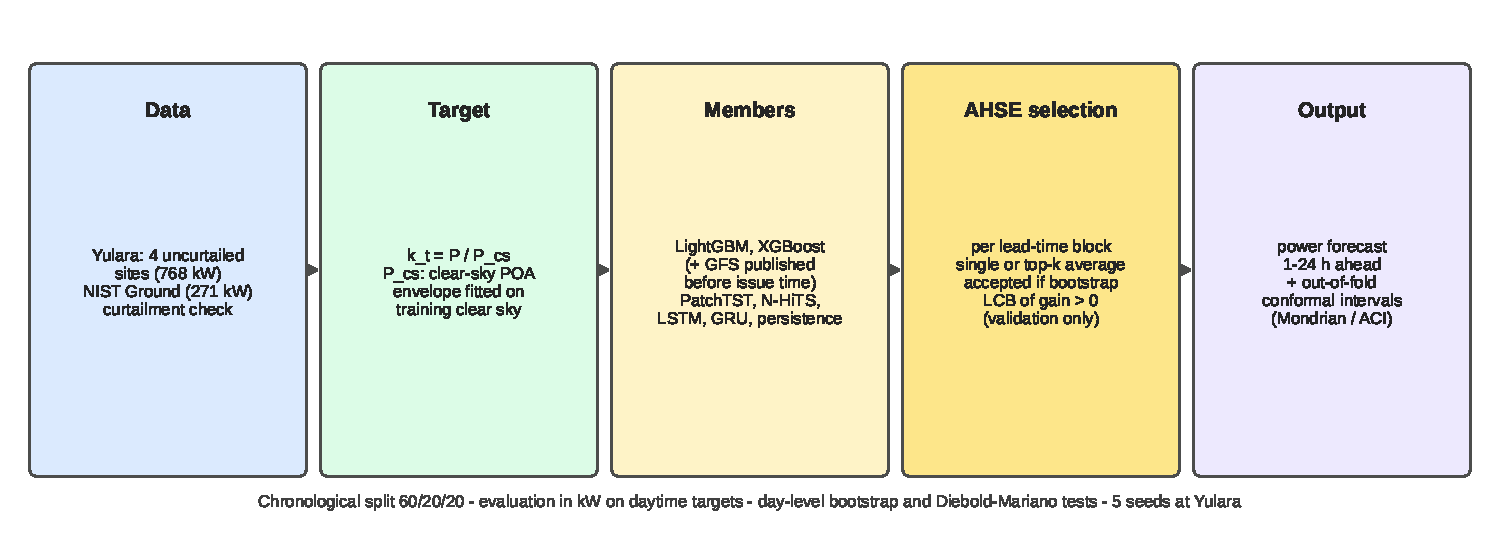
\includegraphics[width=0.95\textwidth]{fig_pipeline.pdf}
\end{graphicalabstract}

%% ------------------------------------------------------------
%% Research Highlights (required by SETA).
%% 3-5 bullets, each a single sentence of at most 85 characters.
%% ------------------------------------------------------------
\begin{highlights}
\item The Yulara series of earlier forecasting studies is curtailed (half of its energy).
\item Benchmark rebuilt on uncurtailed sites and a second climate, evaluated in power.
\item Per-horizon ensemble selection accepts a combination only under a bootstrap guard.
\item Archived GFS forecasts used without look-ahead cut the MAE by 13--26\%.
\item Out-of-fold conformal intervals reach nominal coverage; GFS narrows them by 17\%.
\end{highlights}

\begin{keyword}
Solar power forecasting \sep
Ensemble selection \sep
Numerical weather prediction \sep
Conformal prediction \sep
Curtailment \sep
Off-grid microgrid \sep
Forecast evaluation
\end{keyword}

\end{frontmatter}

%% ============================================================
\section{Introduction}
\label{sec:intro}
% ============================================================
% 01_introduction.tex  (revised 2026-10)
% ============================================================

Global energy systems are being reshaped by the diffusion of solar photovoltaic (PV) generation.
Cumulative PV capacity reached approximately $1{,}865~\mathrm{GW}$ by the end of~2024, with a
record $452~\mathrm{GW}$ added during that year~\cite{irena2025}. In large interconnected grids,
forecast errors are absorbed by reserves and markets; in small and off-grid microgrids, where PV
competes with a few thermal generators, they translate directly into spinning reserve, fuel
consumption and curtailment. Forecasts covering the next hours to the next day are therefore an
operational input of microgrid dispatch.

Machine-learning forecasters and their ensembles are routinely reported to outperform single
models, but three aspects of their evaluation are often fragile. First, the combination strategy
or meta-learner is sometimes fitted on the period used for the final scores, which inflates the
reported gains~\cite{kaufman2012leakage,kapoor2023leakage}. Second, the measured PV output is
taken as the physical resource although it may include operator decisions such as curtailment.
Third, gains are frequently reported on normalised targets, a single seed and a single site,
without tests that account for the strong dependence between overlapping multi-step forecasts.

This paper revisits the Adaptive Honest Selection Ensemble (AHSE), first proposed for the Yulara
plant in Australia, with these issues in mind. We found that the Yulara series used in earlier
studies, including the first version of this work, is the output of a site that is curtailed
around noon; the corresponding claims are withdrawn and the study is rebuilt on uncurtailed data.
The contributions are:

\begin{enumerate}
  \item \textbf{A curtailment-aware benchmark.} We document the curtailment of the Desert Gardens
  site from the public per-site data (about half of its available energy), and use the four
  uncurtailed sites of the same mini-grid as target, with a second, grid-connected site in a
  humid subtropical climate (NIST, USA) obtained from a public data lake.

  \item \textbf{Honest per-horizon-block selection.} AHSE selects, for each block of lead times,
  a single model or an average of the best models, and accepts a combination only when the lower
  bound of a day-level bootstrap interval of its validation gain is positive. All decisions use
  the validation period only.

  \item \textbf{Leak-free weather forecasts.} Archived GFS forecasts enter the tree members and
  the candidate pool using only the run published before the issue time, with a conservative
  five-hour delay.

  \item \textbf{Calibrated uncertainty.} Out-of-fold, Mondrian and adaptive conformal intervals
  are calibrated without touching the test period, optionally by a weather-forecast variable.

  \item \textbf{Transparent evaluation.} Errors in power and as a share of capacity, a
  squared-error skill score against day-ahead persistence, five seeds, day-level bootstrap and
  Diebold--Mariano tests, and a sensitivity analysis of the validation design; all scripts and
  result tables are public.
\end{enumerate}

Section~\ref{sec:related} reviews related work. Section~\ref{sec:methodology} defines the
forecasting task, the selection protocol, the use of weather forecasts and the prediction
intervals. Section~\ref{sec:setup} describes the sites, the curtailment analysis and the
evaluation protocol. Section~\ref{sec:results} reports and discusses the results and
Section~\ref{sec:conclusion} concludes.

\FloatBarrier

%% ============================================================
\section{Related Work}
\label{sec:related}
% ============================================================
% 02_related_work.tex
% AHSE — Adaptive Honest Selection Ensemble
% for Multi-Horizon PV Power Forecasting
% Target journal: Sustainable Energy Technologies and Assessments (SETA)
% ============================================================

This section reviews four lines of work on which AHSE builds:
learning architectures for PV forecasting, ensemble methods for energy
time series, the clearness index as a normalised target, and the use of
weather forecasts and prediction intervals.

% ------------------------------------------------------------
\subsection{Machine learning and deep learning for PV forecasting}
\label{subsec:rw_ml_dl}

Data-driven approaches now dominate short-term PV forecasting, and
recent reviews confirm the shift away from physical and statistical
models towards machine-learning and deep-learning
pipelines~\cite{gupta2025state,kumardhaked2025exploring,yu2024ref,chandel2023techniques}.
Two families coexist within this paradigm. Gradient-boosting decision
tree (GBDT) models such as LightGBM~\cite{ke2017lightgbm} and
XGBoost~\cite{chen2016xgboost}---both rooted in Friedman's gradient
boosting framework~\cite{friedman2001greedy}---train rapidly, tolerate
missing and noisy features, and remain competitive on datasets of
moderate size. Matera~\textit{et~al.}~\cite{matera2023hourly} confirm
this by showing that ambient meteorological variables fed into a
network of shallow artificial neural networks already deliver
competitive hourly forecasts across multiple latitudes, indicating that
strong PV performance does not necessarily require deep architectures.
On the deep-learning side, recurrent networks
(LSTM~\cite{hochreiter1997lstm}, GRU~\cite{cho2014gru}) were the first
popular choice for sub-hourly lead times but lose effective memory
beyond one diurnal cycle~\cite{coya2025accuracy}, whereas
Transformer-based~\cite{vaswani2017attention} PatchTST~\cite{nie2023patchtst}
and the hierarchical MLP model N-HiTS~\cite{challu2023nhits} improve
long-horizon accuracy through input patching and multi-rate
interpolation, at the cost of longer training and weaker performance
on small datasets~\cite{suresh2025benchmarking,wang2025patchtst}.
Dimitriadis~\textit{et~al.}~\cite{dimitriadis2025deep} further show
that a deep model trained across interconnected countries must
explicitly handle distribution shift to preserve accuracy, and Luo and
Zhang~\cite{luo2022adaptive} reach a similar conclusion through a
concept-drift-triggered adaptive LSTM in which re-training fires
whenever the statistical properties of the incoming data shift.
Hybrid combinations of these families~\cite{cisse2026optimized,hou2024ref,abumohsen2024combining}
further illustrate that no single base architecture is universally
optimal. These studies share one structural limitation: a single
monolithic model is asked to serve every atmospheric regime, even
though no architecture has been shown to dominate across both stable
clear-sky and variable cloud-dominated conditions.

% ------------------------------------------------------------
\subsection{Ensemble methods for energy forecasting}
\label{subsec:rw_ensemble}

Ensembles are the natural response to regime sensitivity. Simple
averaging, inverse-error weighting and Ridge-based stacking reliably
reduce variance relative to the best single model and have been widely
applied to PV forecasting in hybrid
frameworks~\cite{cisse2026optimized,hou2024ref,perera2024regional,abumohsen2024combining},
including the Yulara plant in the Northern Territory of
Australia~\cite{cisse2026optimized} (prior work by the present
authors); however, that study's hybrid component weights remain nearly
fixed at inference, preventing real reallocation of predictive
authority when the regime shifts within minutes. The present work
addresses this limitation by introducing a validation-only selection
protocol that dynamically activates or deactivates the ensemble. Dynamic
ensemble selection (DES), initially developed for general classifier
combination~\cite{cruz2018dynamic}, addresses this by adapting weights
online, either through local-competence metrics in feature space or
through learned gating networks and reinforcement
modules~\cite{zhang2024interpretable,song2025dynamic,achouri2026dynamic,konduru2025irradiance}.
Santos~\textit{et~al.}~\cite{santos2022irradiance} apply DES directly
to solar irradiance forecasting and report statistically significant
gains over static ensembles, confirming the practical value of
regime-aware model switching. Two recurring issues persist across the
DES literature, however. First, a non-trivial share of reported gains
stems from \emph{information leakage}: the combination strategy or
meta-learner is fit on the same temporal partition used for final
evaluation, which inflates performance and undermines
reproducibility~\cite{kaufman2012leakage,kapoor2023leakage}. Second,
very few studies include an explicit \emph{guard} preventing ensemble
activation when a single model already dominates; without such a
guard, an ensemble can be selected purely because it happens to match
the test partition, a symptom of selection overfitting that only
becomes visible once the model is deployed. These two issues motivate
the validation-only, statistically guarded selection introduced in
Section~\ref{sec:methodology}.

% ------------------------------------------------------------
\subsection{Clearness index and curtailment}
\label{subsec:rw_kt}

Physics-informed features offer an alternative to learned regime
detectors~\cite{pombo2022benchmarking,mayer2021extensive}. The
clearness index \(k_t = G_\mathrm{GHI}/G_\mathrm{cs}\) normalises
measured global horizontal irradiance by the clear-sky baseline
produced by models such as Ineichen--Perez~\cite{ineichen2002broadband},
here implemented via pvlib-python~\cite{holmgren2018pvlib}. This
normalisation removes the deterministic diurnal and seasonal cycles
and isolates the stochastic component driven by cloud dynamics;
Voyant~\textit{et~al.}~\cite{voyant2025importance} show that the
choice of clear-sky model materially affects short-term forecasting
accuracy, and Lauret~\textit{et~al.}~\cite{lauret2022forecasts}
demonstrate that solar forecasts built on the clear-sky index
systematically outperform those built on raw irradiance. The clear-sky reference of a PV
\emph{power} series must describe the array rather than the horizontal
irradiance: when the measured output is limited by an inverter or by
the operator, the clearness index saturates and no longer reflects the
sky. Curtailment is common in weak grids and off-grid systems, yet
public benchmarks rarely check for it.

% ------------------------------------------------------------
\subsection{Weather forecasts and prediction intervals}
\label{subsec:rw_nwp}

Beyond a few hours, statistical forecasts based on past observations
lose skill quickly and numerical weather prediction (NWP) becomes the
main source of information~\cite{mayer2021extensive,pombo2022benchmarking}.
Using NWP in a fair evaluation requires archived forecasts that were
actually available at the issue time; analyses or forecasts from later
runs leak future information. On the uncertainty side, probabilistic
PV forecasting is increasingly
studied~\cite{xiong2025probabilistic}, and conformal prediction offers
distribution-free intervals around any point
forecaster~\cite{vovk2005algorithmic,barber2021jackknife}; adaptive
conformal inference~\cite{gibbs2021adaptive} relaxes the
exchangeability assumption and has been applied to hour-ahead PV
forecasting with Transformers~\cite{suresh2025benchmarking}. Calibrating
intervals around a \emph{selected} ensemble raises the same leakage
issue as the selection itself, since in-sample validation residuals
are optimistic.

% ------------------------------------------------------------
\subsection*{Positioning of AHSE}
\label{subsec:rw_positioning}

AHSE differs from the dynamic ensembles reviewed above in three ways.
Its selection is made per block of lead times, uses the validation
period only and accepts a combination only when a day-level bootstrap
interval of the gain excludes zero, so that it falls back to the best
single model when the evidence is weak. Archived weather forecasts are
used with an explicit publication delay. Prediction intervals are
calibrated out-of-fold with respect to the selection. Unlike earlier
studies of the Yulara plant~\cite{cisse2026optimized}, including the
first version of this work, the target is checked for curtailment and
the evaluation is reported in power, on two sites, over several seeds.


\FloatBarrier

%% ============================================================
\section{Methodology}
\label{sec:methodology}
% ============================================================
% 03_methodology.tex  (revised 2026-10; written from the code of this repository)
% ============================================================

This section defines the forecasting task, the target normalisation, the base models, the
honest per-horizon-block selection that constitutes AHSE, the leak-free use of archived weather
forecasts and the conformal prediction intervals. Every quantity that is fitted or selected uses
the training or validation partitions only; the test partition is used once, for the final
scores.

% ------------------------------------------------------------
\subsection{Forecasting task}
\label{subsec:task}

Data are hourly means on a complete local-time grid, each value labelled by the start of its
interval. A forecast is issued every hour at the time $t_0$ of the last observation and predicts
the next $H = 24$ hourly values, i.e.\ lead times from 1 to 24~h (intraday to day-ahead). Inputs
are the $L = 24$ preceding hours of 15 features: the clearness index $k_t$ (defined below),
measured global horizontal irradiance, temperature, wind speed and direction, pressure, solar
zenith angle, clear-sky GHI and cyclic encodings of hour, month, day of year and weekday. A
sequence is discarded if its input or target window touches a data gap longer than one hour;
shorter gaps are interpolated linearly.

% ------------------------------------------------------------
\subsection{Clear-sky power and clearness index}
\label{subsec:pcs}

The target is the clearness index of the PV output, $k_t = P / P_\mathrm{cs}$, clipped to
$[0, 1.5]$ and set to zero at night. Its denominator describes the clear-sky output of the array:
\begin{equation}
  P_\mathrm{cs}(t) = \min\bigl\{c\,G^\mathrm{cs}_\mathrm{POA}(t;\beta,\gamma),\; P_\mathrm{max}\bigr\},
  \label{eq:pcs}
\end{equation}
where $G^\mathrm{cs}_\mathrm{POA}$ is the clear-sky plane-of-array irradiance (Ineichen--Perez
clear sky~\cite{ineichen2002broadband}, isotropic transposition,
pvlib~\cite{holmgren2018pvlib}) for tilt $\beta$ and azimuth $\gamma$, $c$ a scale factor and
$P_\mathrm{max}$ the 99.9th percentile of the training output (inverter limit). $(\beta, \gamma)$
are chosen on a grid ($\beta \in \{0, 5, \dots, 45\}^\circ$, $\gamma$ in steps of $30^\circ$) and
$c$ is the median ratio of power to $G^\mathrm{cs}_\mathrm{POA}$ over clear-sky instants of the
training period only (solar zenith below $75^\circ$ and measured GHI within $\pm10\%$ of the
clear-sky GHI). Equation~\eqref{eq:pcs} is a power envelope, not an identification of the array
geometry: at NIST it selects $\beta = 35^\circ$ for an array tilted at $20^\circ$, with a median
relative error of 6\% on clear-sky instants (4\% at Yulara). All forecasts are converted back to
power, $\hat P = \hat k_t \, P_\mathrm{cs}$, for evaluation.

% ------------------------------------------------------------
\subsection{Base models}
\label{subsec:base}

The pool contains two gradient-boosted tree models, LightGBM~\cite{ke2017lightgbm} and
XGBoost~\cite{chen2016xgboost} (one regressor per lead time on the flattened input window,
1{,}000 trees, learning rate 0.05, no early stopping), four neural multi-output forecasters,
PatchTST~\cite{nie2023patchtst}, N-HiTS~\cite{challu2023nhits}, LSTM~\cite{hochreiter1997lstm}
and GRU~\cite{cho2014gru} (early stopping on the validation loss), and two references: last-value
persistence of $k_t$ and day-ahead persistence, which forecasts $k_t(t_0 + h)$ by the value
observed 24~h earlier. Hyper-parameters are fixed in the configuration files of the repository
and were not tuned on the test period.

% ------------------------------------------------------------
\subsection{Honest per-horizon-block selection (AHSE)}
\label{subsec:hbs}

Errors grow with the lead time and the ranking of the base models changes with it. AHSE
therefore selects a forecast separately for blocks of lead times
$\mathcal{B} = \{[1\,\mathrm{h}],\ (1, 6\,\mathrm{h}],\ (6, 24\,\mathrm{h}]\}$, using the
validation partition only and daytime targets only, exactly as in the final evaluation.
\begin{enumerate}
  \item The reference $r$ is the single model with the lowest validation MAE over all lead
        times.
  \item For each block $b$, the candidates are every single model and the averages of the
        $k \in \{2, 3, 4\}$ models with the lowest validation MAE on that block.
  \item A candidate $c$ may replace $r$ on block $b$ only if the lower bound of the one-sided
        95\% bootstrap confidence interval of its validation gain
        $\Delta_b(c) = \mathrm{MAE}_b(r) - \mathrm{MAE}_b(c)$ is positive. Absolute errors are
        summed per forecast day and whole days are resampled with replacement (1{,}000
        replicates), which respects the strong dependence between the overlapping forecasts
        issued on the same day.
  \item Among eligible candidates the one with the lowest validation MAE is kept; if none is
        eligible, the block keeps the reference.
\end{enumerate}
The guard makes the selection conservative: AHSE combines models only where the validation
evidence of a gain is statistically clear, and otherwise falls back to the best single model.
For comparison we also report \emph{AHSE-global}, the selector of the original version of this
work, which chooses one strategy for all lead times (best model, average, stacking or a
clearness-index gate) with a fixed minimum-improvement threshold of 0.5\% on all validation
samples.

% ------------------------------------------------------------
\subsection{Archived weather forecasts without look-ahead}
\label{subsec:nwp}

Archived forecasts of the Global Forecast System (GFS, 0.25$^\circ$, runs at 00, 06, 12 and
18~UTC~\cite{ncep2015gfs}) provide the downward shortwave radiation at the surface and the total
cloud cover, interpolated bilinearly to the site. GFS stores averages from the start of each
6-hour cycle; 3-hour means over $(v - 3\,\mathrm{h}, v]$ are recovered as
$\bar x_{(v-3, v]} = 2\,\bar x_{(v-6, v]} - \bar x_{(v-6, v-3]}$ in the second half of the cycle.
A forecast issued at $t_0$ may only use the latest run that was \emph{published} by $t_0$,
\begin{equation}
  \mathrm{run}(t_0) = \max\{\tau : \tau + \delta \le t_0\}, \qquad \delta = 5\,\mathrm{h},
  \label{eq:run}
\end{equation}
a conservative delay (GFS products are usually available 3.5--4.5~h after the initial time).
Each target interval $[t, t + 1\,\mathrm{h})$ takes the 3-hour window that contains its
midpoint. For every lead time the tree models receive the GFS radiation, the cloud cover, the
clear-sky GHI and a GFS clearness index, defined as the GFS radiation divided by the clear-sky GHI
averaged over the \emph{same} 3-hour window (dividing a 3-hour mean by an instantaneous clear sky
distorts mornings and evenings). The GFS clearness index is also offered to the selector as a
stand-alone candidate, with day-ahead persistence as fallback when the archive has no value. The
neural members receive no weather forecast, so that runs with and without GFS differ only by
this information.

% ------------------------------------------------------------
\subsection{Conformal prediction intervals}
\label{subsec:conformal}

Point forecasts are complemented by distribution-free intervals. Conformity scores are the
absolute $k_t$ residuals of daytime targets. Because the selector is fitted on the validation
partition, its validation residuals would be optimistic; calibration therefore uses out-of-fold
forecasts obtained by refitting the selector on four of five contiguous folds of validation days
and predicting the fifth, in the spirit of cross-validation conformal
methods~\cite{barber2021jackknife}. Scores are calibrated separately (Mondrian
conformal~\cite{vovk2005algorithmic}) in each cell formed by a block of lead times and a bin of a
variable known at the issue time: by default the predicted $k_t$ (below 0.4, 0.4--0.8, above
0.8); with GFS, alternatively the GFS clearness index (validation tertiles). The half-width for
level $1-\alpha$ is the $\lceil (n+1)(1-\alpha) \rceil$-th smallest of the $n$ scores of the
cell. Since exchangeability is questionable for weather-driven series, we also apply adaptive
conformal inference~\cite{gibbs2021adaptive}: the miscoverage level used on day $d$ is
$\alpha_d = \alpha_{d-1} + \eta\,(\alpha - e_{d-2})$, where $e_{d-2}$ is the share of
non-covered targets of the forecasts issued two days earlier, whose horizons are entirely observed
at the time of the update ($\eta = 0.02$, $\alpha_d \in [0.01, 0.5]$). Intervals are assessed by
coverage, mean width and the interval score
$W + \tfrac{2}{\alpha}\bigl[(\ell - y)_+ + (y - u)_+\bigr]$.

\FloatBarrier

%% ============================================================
\section{Data Description and Experimental Configuration}
\label{sec:setup}
% ============================================================
% 04_experimental_setup.tex  (revised 2026-10)
% ============================================================

% ------------------------------------------------------------
\subsection{Yulara: a curtailed off-grid mini-grid}
\label{subsec:yulara}

The Yulara installation (Northern Territory, Australia; $25.24^\circ$\,S, $131.04^\circ$\,E,
492~m, hot desert climate) consists of five PV sites (1.8~MW in total) feeding the
gas-supplied mini-grid of the Ayers Rock Resort; per-site 5-min measurements and a shared
weather station are published by the DKA Solar Centre~\cite{dkasc_yulara}. The series used in
earlier work on this plant, including the first version of the present study, is exactly the
output of the largest site, Desert Gardens (1{,}058~kW). A site-by-site analysis shows that this
site is systematically curtailed around solar noon (Fig.~\ref{fig:curtailment}): under high
irradiance its output relative to the other sites falls to 0.37 at noon while the four other
sites stay between 0.98 and 1.07, and on clear days the total PV output is held at
615--630~kW between 11:00 and 15:00. Treating curtailment as censoring of the available power
(delivered $=\min$(available, cap)) and reconstructing the available power from the
uncurtailed sites, we estimate that 50.6\% of the energy available at Desert Gardens was
curtailed (conservative bounds 31.7--59.1\%; 36--39\% in summer, 56--65\% from April to
September). These figures are inferred from the data; the control logic has not been confirmed
by the operator.

A curtailed series mixes weather and dispatch decisions: its $k_t$ saturates at the
curtailment cap instead of the clear-sky envelope, and a forecaster trained on it learns the
dispatch rule. The forecasting target is therefore the summed output of the four uncurtailed
sites (Service Station 227~kW, Sails in the Desert 107~kW, Laundry 328~kW and Connellan Airport
106~kW; 768~kW in total) from 2 April 2016 to 13 May 2020, after which these sites stop
reporting for six months while Desert Gardens keeps operating.

\begin{figure}[t]
  \centering
  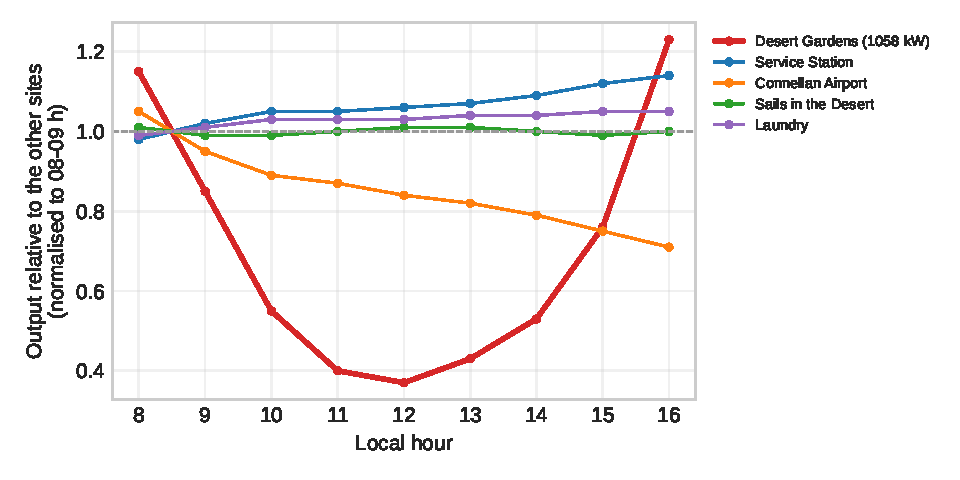
\includegraphics[width=0.85\linewidth]{fig_curtailment.pdf}
  \caption{Output of each Yulara site relative to the others under high irradiance, by hour of
  the day (normalised to 08--09~h). Desert Gardens, the series used in earlier studies, falls to
  0.37 of its expected share at noon; Connellan Airport's monotone afternoon decline is an
  orientation effect.}
  \label{fig:curtailment}
\end{figure}

% ------------------------------------------------------------
\subsection{NIST: a grid-connected array in a humid subtropical climate}
\label{subsec:nist}

The second site is the Ground array of the NIST campus in Gaithersburg, Maryland, USA
($39.13^\circ$\,N, $77.21^\circ$\,W, 138~m; K\"oppen Cfa), 271~kW$_\mathrm{DC}$, south-facing,
tilted at $20^\circ$~\cite{boyd2017nist}. Its 1-min inverter AC power and the array's own
sensors (horizontal thermopile pyranometer, ambient temperature, wind) were obtained from the
public PVDAQ data lake (system 4902, NIST\_Ground\_1)~\cite{deline2021pvdaq}, whose values are
identical to the NIST archive for the overlapping year 2016, except the pyranometer, stored in
millivolts. Its conversion to W\,m$^{-2}$ follows NIST's own constants (one change in May 2016,
reproduced exactly from the NIST archive); the raw signal drops by about 16\% between 10 and
17~October~2017 while the calibrated reference cell stays consistent with the AC power, which
indicates a sensor change with an unknown constant. The series is therefore restricted to
1~January~2016 -- 10~October~2017. An inverter outage (21~June -- 5~July~2016, 524~h) is
excluded by the gap rule. Pressure is not measured at the array and is set to the standard
pressure of the altitude (a constant feature).

% ------------------------------------------------------------
\subsection{Weather forecasts}
\label{subsec:gfs_data}

GFS forecasts were retrieved from the NSF NCAR Geoscience Data Exchange (dataset
d084001~\cite{ncep2015gfs}) as monthly subsets of all runs with forecast hours up to 48~h, for
April~2016 -- May~2020 at Yulara and January~2016 -- December~2018 at NIST. Every target of
every test forecast has a GFS value from the run selected by Eq.~\eqref{eq:run}; 0.1\% of the
NIST training and validation targets have none (the tree models handle these missing values
natively).

% ------------------------------------------------------------
\subsection{Partitions, runs and reproducibility}
\label{subsec:partitions}

Each series is split chronologically into training, validation and test partitions (60/20/20\%
of the rows; Table~\ref{tab:partitions}). The test partition contains only forecasts issued after
the end of the validation period. Every configuration is run with and without GFS; the neural
members of the run with GFS are the checkpoints of the run without GFS, so that the two runs
differ only by the GFS information. At Yulara, five seeds (42, 1, 2, 3, 4) control the neural
networks and the tree models. As a sensitivity analysis, a season-balanced validation keeps the
same test partition but uses every fourth week of the preceding period as validation, dropping
sequences whose window mixes training and validation rows. Data preparation, models, selection,
evaluation and every table of this paper are produced by the scripts and configuration files of
the public repository.

\begin{table}[t]
  \centering
  \caption{Data partitions (first and last target day of the forecasts in each partition;
  number of hourly forecasts issued, each with 24 lead times).}
  \label{tab:partitions}
  \small
  \begin{tabular}{lllll}
    \toprule
    Site & Capacity & Training & Validation & Test \\
    \midrule
    Yulara (4 sites) & 768 kW & 2016-04-03 -- 2018-09-19 & 2018-09-21 -- 2019-07-17 & 2019-07-19 -- 2020-05-13 \\
                     &        & 19{,}847 & 5{,}699 & 6{,}650 \\
    NIST Ground      & 271 kW & 2016-01-02 -- 2017-01-23 & 2017-01-25 -- 2017-06-02 & 2017-06-04 -- 2017-10-10 \\
                     &        & 8{,}155 & 3{,}040 & 3{,}069 \\
    \bottomrule
  \end{tabular}
\end{table}

% ------------------------------------------------------------
\subsection{Evaluation}
\label{subsec:evaluation}

Forecasts are evaluated in power, $\hat P = \hat k_t P_\mathrm{cs}$, against the measured
power, on daytime targets ($P_\mathrm{cs}$ above the night threshold; measured zero output by day
is negligible, 2 of 15{,}671 hours above $10^\circ$ elevation at Yulara). We report the MAE and
RMSE in kW and as a percentage of the DC capacity (nMAE, nRMSE), and the skill score
$1 - \mathrm{MSE}/\mathrm{MSE}_\mathrm{ref}$ against day-ahead persistence. The coefficient of
determination of the power is high for every model because the diurnal cycle dominates it
(0.84 for day-ahead persistence at Yulara) and discriminates little between models; MAE in
$k_t$ units is given in the supplementary tables only, because it weighs dawn and dusk hours,
where $k_t$ is noisy and the power small, as much as midday hours and can reverse the ranking of
close models.

Forecasts issued on the same day share most of their targets, so losses are first averaged per
issue day. Differences between two forecasts are assessed with a bootstrap over days (95\%
interval of the MAE difference, 5{,}000 replicates) and a Diebold--Mariano
test~\cite{diebold1995comparing} on the daily loss differentials with a Newey--West
variance~\cite{newey1987simple}.

\FloatBarrier

%% ============================================================
\section{Results and Discussion}
\label{sec:results}
% ============================================================
% 05_results.tex  (revised 2026-10; numbers from results/power_summary and the run tables)
% ============================================================

\subsection{Point forecasts}
\label{subsec:res_point}

Tables~\ref{tab:yulara} and~\ref{tab:nist} report the test errors in power. At Yulara the values
are means and standard deviations over five seeds; at NIST a single seed is reported.

\begin{table}[t]
  \centering
  \caption{Yulara (four uncurtailed sites, 768~kW), test period 2019-07-19 -- 2020-05-13, lead
  times 1--24~h, daytime targets. Mean $\pm$ standard deviation over five seeds. Skill: MSE
  skill score against day-ahead persistence.}
  \label{tab:yulara}
  \small
  \begin{tabular}{lcccccc}
    \toprule
    & \multicolumn{3}{c}{without GFS} & \multicolumn{3}{c}{with GFS} \\
    \cmidrule(lr){2-4}\cmidrule(lr){5-7}
    Model & MAE (kW) & nRMSE (\%) & Skill & MAE (kW) & nRMSE (\%) & Skill \\
    \midrule
    AHSE                   & \textbf{36.18 $\pm$ 0.32} & \textbf{8.21} & \textbf{0.36} & \textbf{31.32 $\pm$ 0.05} & \textbf{6.95} & \textbf{0.54} \\
    AHSE-global            & 37.37 $\pm$ 0.48 & 8.23 & 0.36 & 31.34 $\pm$ 0.06 & 6.95 & 0.54 \\
    XGBoost                & 41.35 $\pm$ 0.12 & 8.61 & 0.30 & 31.34 $\pm$ 0.06 & 6.95 & 0.54 \\
    LightGBM               & 42.07 $\pm$ 0.07 & 8.76 & 0.27 & 32.36 $\pm$ 0.03 & 7.08 & 0.53 \\
    PatchTST               & 40.02 $\pm$ 0.89 & 8.77 & 0.27 & -- & -- & -- \\
    N-HiTS                 & 40.62 $\pm$ 1.17 & 8.86 & 0.25 & -- & -- & -- \\
    GRU                    & 40.41 $\pm$ 0.94 & 8.62 & 0.30 & -- & -- & -- \\
    LSTM                   & 42.50 $\pm$ 1.77 & 9.10 & 0.22 & -- & -- & -- \\
    GFS clearness index    & -- & -- & -- & 46.54 & 9.58 & 0.13 \\
    Day-ahead persistence  & 40.56 & 10.27 & 0 & 40.56 & 10.27 & 0 \\
    \bottomrule
  \end{tabular}

  \smallskip
  \footnotesize The neural members do not use GFS; their errors are identical in both columns.
\end{table}

\begin{table}[t]
  \centering
  \caption{NIST Ground array (271~kW), test period 2017-06-04 -- 2017-10-10, lead times
  1--24~h, daytime targets, seed 42.}
  \label{tab:nist}
  \small
  \begin{tabular}{lcccccc}
    \toprule
    & \multicolumn{3}{c}{without GFS} & \multicolumn{3}{c}{with GFS} \\
    \cmidrule(lr){2-4}\cmidrule(lr){5-7}
    Model & MAE (kW) & nRMSE (\%) & Skill & MAE (kW) & nRMSE (\%) & Skill \\
    \midrule
    AHSE                   & \textbf{27.55} & \textbf{14.52} & \textbf{0.41} & \textbf{20.39} & \textbf{10.80} & \textbf{0.68} \\
    AHSE-global, XGBoost   & 27.84 & 14.79 & 0.39 & 20.47 & 10.81 & 0.68 \\
    LightGBM               & 28.47 & 15.26 & 0.35 & 20.79 & 11.06 & 0.66 \\
    GRU                    & 28.89 & 14.75 & 0.39 & -- & -- & -- \\
    LSTM                   & 29.67 & 15.06 & 0.37 & -- & -- & -- \\
    PatchTST               & 29.97 & 15.87 & 0.30 & -- & -- & -- \\
    N-HiTS                 & 30.51 & 15.67 & 0.32 & -- & -- & -- \\
    GFS clearness index    & -- & -- & -- & 28.63 & 14.26 & 0.43 \\
    Day-ahead persistence  & 34.13 & 18.96 & 0 & 34.13 & 18.96 & 0 \\
    \bottomrule
  \end{tabular}
\end{table}

\paragraph{Weather forecasts are the main source of skill.}
Adding GFS covariates lowers the MAE of AHSE from 36.18 to 31.32~kW at Yulara (nMAE 4.71\%
$\to$ 4.08\%) and from 27.55 to 20.39~kW at NIST (10.17\% $\to$ 7.52\%). The gain is significant
for every seed at Yulara (4.4 to 5.2~kW; Diebold--Mariano statistic 3.2--3.8 on daily losses) and
at NIST (7.17~kW, 95\% interval [5.51, 8.92]~kW, DM 5.7). It is larger in the humid subtropical
climate of Maryland, where the clearness index is far less persistent from one day to the next
than in the desert, and it grows with the lead time (Fig.~\ref{fig:leadtime}): past observations
only inform the first hours, whereas the weather forecast carries information for the whole
horizon. Used alone, the GFS clearness index is worse than day-ahead persistence at Yulara and
better at NIST; its value comes from the learned combination with recent observations.

\begin{figure}[t]
  \centering
  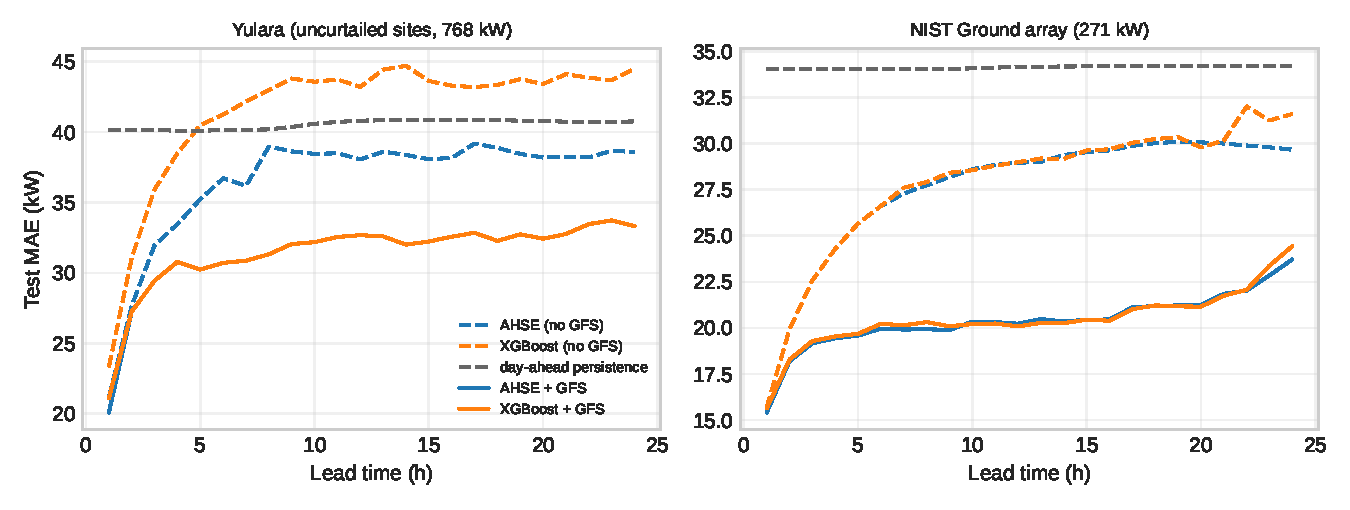
\includegraphics[width=\linewidth]{fig_mae_leadtime.pdf}
  \caption{Test MAE in kW by lead time, without GFS (dashed) and with GFS (solid), seed 42. Day-ahead
  persistence is shown for reference.}
  \label{fig:leadtime}
\end{figure}

\paragraph{AHSE combines models only when the evidence supports it.}
Without GFS at Yulara, the selector keeps N-HiTS as reference and combines models on every block
(LightGBM, XGBoost and N-HiTS on the first hour; four models on 1--6~h; day-ahead persistence,
N-HiTS and XGBoost beyond 6~h). AHSE then beats the best single model of every seed, which is
N-HiTS, GRU or PatchTST depending on the seed, by 2.8 to 3.9~kW (7 to 10\%; DM 5.0--7.2), and
AHSE-global by 1.2~kW on average. With GFS, the GFS-fed XGBoost dominates the pool: the guard keeps
it alone from the second hour on, and AHSE equals it (differences of at most 0.05~kW). At NIST,
AHSE is not significantly different from XGBoost, with or without GFS (gains of 0.28 and
0.08~kW, $p = 0.22$ and $0.48$), and is significantly better than LightGBM. AHSE is therefore
never significantly worse than the best member chosen in hindsight on the test set; it improves
on it when the pool contains complementary members and falls back to it otherwise. The seed
variability of AHSE (0.32~kW without GFS, 0.05~kW with GFS) is an order of magnitude smaller
than these differences.

\paragraph{A metric caveat.}
At Yulara without GFS, day-ahead persistence has a lower MAE (40.6~kW) than XGBoost and LightGBM,
but a much larger RMSE (10.3\% against 8.6\% of capacity): in a sunny desert the clearness index
is very persistent and the MAE rewards forecasts that are exact on most days and badly wrong on
the few cloudy ones. Conversely, a MAE computed on $k_t$ instead of power gives the same weight
to dawn and dusk hours as to noon; on that scale AHSE appeared significantly behind XGBoost at
NIST without GFS, a difference that disappears in power. Conclusions should therefore rest on
power errors and include a squared-error measure.

% ------------------------------------------------------------
\subsection{Prediction intervals}
\label{subsec:res_intervals}

\begin{table}[t]
  \centering
  \caption{90\% prediction intervals of AHSE on the test period ($k_t$ units; out-of-fold
  calibration on the validation period). IS: interval score (lower is better).}
  \label{tab:intervals}
  \small
  \begin{tabular}{llccc}
    \toprule
    Configuration & Method & Coverage & Width & IS \\
    \midrule
    Yulara, no GFS & split, pooled            & 0.909 & 0.604 & 0.864 \\
                   & split, Mondrian          & 0.910 & 0.525 & 0.800 \\
                   & adaptive (ACI), Mondrian & 0.901 & 0.495 & 0.805 \\
    Yulara, GFS    & split, pooled            & 0.903 & 0.491 & 0.728 \\
                   & split, Mondrian          & 0.907 & 0.420 & 0.657 \\
                   & adaptive (ACI), Mondrian & 0.902 & 0.413 & 0.656 \\
                   & split, binned by GFS     & 0.916 & 0.440 & \textbf{0.627} \\
    NIST, GFS      & split, Mondrian          & 0.921 & 0.790 & 1.002 \\
                   & adaptive (ACI), Mondrian & 0.910 & 0.750 & 0.998 \\
                   & split, binned by GFS     & 0.907 & 0.690 & \textbf{0.949} \\
    \bottomrule
  \end{tabular}
\end{table}

All calibrated intervals reach their nominal coverage on the test period
(Table~\ref{tab:intervals}). At Yulara, Mondrian calibration by lead-time block and forecast
level lowers the interval score by 7--10\% against pooled calibration and adaptive conformal
inference brings the coverage closest to the nominal level; at NIST the Mondrian cells do not
improve on pooled calibration (interval score 1.002 against 0.998). GFS narrows the 90\%
intervals by 17\% at Yulara (0.413 against 0.495 with ACI). Binning the calibration by the GFS
clearness index, a quantity known at the issue time, gives the best interval score at both sites
and raises the coverage on variable days (0.82 against 0.77 at Yulara). Coverage remains below
nominal on overcast and variable days (0.62--0.82 at Yulara, depending on the configuration and
the method), a
limitation shared by marginal conformal methods when the conditioning event is defined by the
outcome.

% ------------------------------------------------------------
\subsection{Sensitivity analyses}
\label{subsec:res_sensitivity}

\paragraph{Season-balanced validation.}
With the season-balanced validation (Section~\ref{subsec:partitions}), the test MAE of AHSE is
38.11 instead of 36.53~kW at Yulara without GFS ($p = 0.015$), 30.86 instead of 31.38~kW with GFS
(n.s.), and 29.16 instead of 27.55~kW at NIST without GFS ($p = 0.05$; 20.33 against 20.39~kW
with GFS, n.s.), all for seed 42. The single tree models improve, because their training weeks
then extend up to the start of the test period, but the selector keeps XGBoost alone and AHSE
loses the benefit of combining members. The chronological protocol is therefore retained.

\paragraph{Foundation model.}
A zero-shot time-series foundation model (Chronos-2, 7-day context) reaches a test MAE of 0.116 in
$k_t$ units at Yulara without GFS, against 0.107 for AHSE, i.e.\ it does not replace a model
trained on the site.

% ------------------------------------------------------------
\subsection{Discussion}
\label{subsec:discussion}

The original claim of this work was that a regime-gated ensemble of six learners outperforms
every single model on Yulara. Three findings revise it. First, the Yulara series used in that
claim is curtailed: forecasting it amounts to forecasting a dispatch rule, and an honest benchmark
must use uncurtailed output or reconstructed available power. Second, once the target is
physical, the ensemble's advantage is real but moderate (7--10\% without weather forecasts at
Yulara, none at NIST), whereas archived numerical weather forecasts, used without look-ahead,
reduce the error by 13\% at Yulara and 26\% at NIST. Third, a statistically guarded selection is
what makes the ensemble safe: it never degraded the best member in our experiments, while the
single-strategy selector of the original version, guarded only by a fixed 0.5\% threshold, was
1.2~kW worse at Yulara without GFS. For an off-grid
mini-grid such as Yulara, the relevant improvement is the GFS-informed forecast together with
calibrated intervals, which size the spinning reserve and the curtailment headroom of the gas
generators directly.

Limitations: one test period per site (10 months at Yulara, 4 months at NIST), a single seed at
NIST, hourly resolution only, and point GFS forecasts rather than an ensemble prediction system.

\FloatBarrier

%% ============================================================
\section{Conclusion and Future Work}
\label{sec:conclusion}
% ============================================================
% 07_conclusion.tex  (revised 2026-10)
% ============================================================

This paper revisited an adaptive ensemble for photovoltaic forecasting with the aim of making
its evaluation honest and reproducible, and extended it with archived weather forecasts and
calibrated prediction intervals. Hourly forecasts for lead times of 1 to 24~h were evaluated in
power on two contrasting sites: the four uncurtailed sites of the Yulara off-grid mini-grid
(hot desert, 768~kW) and the NIST Ground array (humid subtropical, 271~kW).

\paragraph{Key findings.}
\begin{itemize}
  \item The Yulara series used in earlier studies, the Desert Gardens site, is curtailed around
  noon; we estimate that half of its available energy (31.7--59.1\%) was not delivered. Benchmarks
  on such a series forecast a dispatch rule rather than the solar resource.

  \item Archived GFS forecasts, used only when published before the forecast issue time, are the
  main source of skill: they lower the MAE of AHSE by 13\% at Yulara (36.18 $\to$ 31.32~kW,
  significant for each of five seeds) and by 26\% at NIST (27.55 $\to$ 20.39~kW), with gains
  growing with the lead time.

  \item The per-horizon-block selection with a day-level bootstrap guard combines models only
  where the validation evidence supports it. It beats the best single model of every seed by
  7--10\% at Yulara without weather forecasts and, when one member dominates (GFS-fed XGBoost),
  falls back to it; it was never significantly worse than the best member in hindsight.

  \item Out-of-fold, Mondrian and adaptive conformal calibration give 90\% intervals with
  0.90--0.92 coverage on the test periods; weather forecasts narrow them by 17\% at Yulara, and
  calibrating them by the GFS clearness index gives the best interval score at both sites.

  \item Evaluation choices matter: the MAE of the clearness index and the MAE alone can reverse
  the ranking of close models, so results should be reported in power with a squared-error skill
  score and day-level significance tests.
\end{itemize}

\paragraph{Future work.}
The work opens three directions linked to resilient microgrids. First, forecasting the
\emph{available} power of curtailed sites, reconstructed from uncurtailed neighbours, would give
the operator of an off-grid mini-grid the information needed to schedule its gas generators and
storage instead of reproducing past curtailment decisions. Second, ensemble weather predictions
and probabilistic members would allow the prediction intervals to reflect weather uncertainty
directly, for reserve sizing and risk-aware dispatch. Third, the honest selection protocol can be
coupled with physics-informed models of the PV array and the microgrid, to keep the forecasts
consistent with the physical limits that a dispatch controller has to respect.

\FloatBarrier

%% ============================================================
\section*{Acknowledgements}
The authors gratefully acknowledge the Desert Knowledge Australia Solar Centre (DKASC) for public
access to the Yulara data~\cite{dkasc_yulara}, NIST and the NREL PVDAQ team for the NIST array
data~\cite{boyd2017nist,deline2021pvdaq}, and the NSF NCAR Geoscience Data Exchange for the
archived GFS forecasts~\cite{ncep2015gfs}.
Computational resources were provided by the School of Electrical
Engineering at Wuhan University.

\section*{Funding}
This work was supported by the National Key R\&D Program of China,
``Intergovernmental International Science and Technology Innovation
Cooperation'' Key Special Project (Project No.\ 2024YFE0115600).

\section*{Declaration of Competing Interest}
The authors declare that they have no known competing financial
interests or personal relationships that could have appeared to
influence the work reported in this paper.

\section*{CRediT Authorship Contribution Statement}
\textbf{Bilali Boureima Cissé}: Conceptualization, Methodology,
Software, Formal analysis, Investigation, Data curation, Writing --
original draft, Writing -- review \& editing, Visualization.
\textbf{Ghamgeen Izat Rashed}: Supervision, Writing -- review \&
editing, Funding acquisition.

\section*{Data and Code Availability}
The Yulara per-site data are available from the DKASC portal
(\url{https://dkasolarcentre.com.au/download?location=yulara}); the NIST Ground array data from the
PVDAQ data lake (\url{https://doi.org/10.25984/1846021}, system 4902); the GFS archive from NSF NCAR
GDEX (\url{https://doi.org/10.5065/D65D8PWK}). The code, configuration files, data-preparation and
download scripts, and the tables backing every number of this paper are available at
\url{https://github.com/billciss/ahse-paper-v2}.

%% ============================================================
\bibliographystyle{elsarticle-num}
\bibliography{references}

\end{document}
